\chapter{Gradient Matching with Gaussian Processes}
\label{ch-gmgp}

\section{Preliminary}
\label{sec-preliminary}
This section briefly introduces Gaussian process regression \refsectionp{\ref{sec-gpr}}, Kullback-Leibler (KL) divergence \refsectionp{\ref{sec-kl}}, and mean-field variational inference \refsectionp{\ref{sec-vi}} as the essential machine learning topics for the rest of the work.
Formal treatment can be found by following the references listed for each topic.

\subsection{Gaussian process regression}
\label{sec-gpr}

As a nonparametric, kernel-based Bayesian inference technique, Gaussian process regression is a powerful tool for many non-linear regression tasks.
In terms of application, a Gaussian process prior needs first to be specified on the regression function $f(\mvector{x})\colon\R^D\rightarrow\R$. 
After observing data, the prior can be turned into a posterior distribution to make predictions \citep{murphy2012machine}.
The definition of Gaussian process given by \cite{rasmussen2006gaussian} is listed as follow.

\begin{definition}
A \emph{Gaussian process} is a collection of random variables such that any finite subset of it forms a multivariate Gaussian distribution.
\end{definition}

The Gaussian process prior on $f$ is denoted as
\begin{align}
    f(\mvector{x}{}) & \sim \mathcal{GP}(m(\mvector{x}),\ k(\mvector{x},\ \mvector{x}^\prime)) 
    \label{eq-gp}
    \\
    \intertext{where}
    m(\mvector{x}) &= \mathbb{E}[f(\mvector{x})]
    \label{eq-gp-mean-function}
    \\  		
    k(\mvector{x}, \mvector{x}^\prime) &= \mathbb{E}[(f(\mvector{x}) - m(\mvector{x}))(f(\mvector{x}^\prime) - m(\mvector{x}^\prime))]
    \label{eq-gp-cov-function}
\end{align}

The above equations simply mean that for any finite collection of points $\mdata{X} = \{\mvector{x}_i \in \R^D \vert i=\mrange{1}{N}\}$, we have $\mdata{f} \vert \mdata{X} \sim \mathcal{N}(\mdata{m},\ \mdata{K}(\mdata{X},\ \mdata{X}))$, where $\mathrm{f}_i = f(\mvector{x}_i)$, $\mathrm{m}_i = m(\mvector{x}_i)$, and $\mathrm{K}_{ij} = k(\mvector{x}_i, \mvector{x}_j)$ for $i,j=\mrange{1}{N}$.
This shows that a Gaussian process is completely specified by its \emph{mean function} \refequationp{\ref{eq-gp-mean-function}} and \emph{covariance function} \refequationp{\ref{eq-gp-cov-function}}.
Furthermore, to form a multivariate Gaussian distribution, the covariance function must generate a covariance matrix that is positive definite for any set of points.

We often only have access to noisy observations denoted by $\mdata{y} = \{y_i \vert i=\mrange{1}{N}\}$ such that $y_i = f(\mvector{x}_i) + \epsilon_i$ for $i=\mrange{1}{N}$.
We assume i.i.d.\ additive noise $\epsilon \sim \mathcal{N}(0, \sigma^2)$.
For any finite collection of test points $\mdata{X}^* = \{\mvector{x}^*_i \in \R^D \vert i=\mrange{1}{M}\}$, we have
\begin{align}
    \begin{bmatrix}
        \mdata{y} 
        \\ 
        \mdata{f}^*
    \end{bmatrix}
    \sim 
    \mathcal{N}(
        \begin{bmatrix}
            \mdata{m} 
            \\ 
            \mdata{m}^*
        \end{bmatrix}
        ,
        \begin{bmatrix}
            \mdata{K}(\mdata{X}, \mdata{X}) + \sigma^2\mI 
                & \mdata{K}(\mdata{X}, \mdata{X}^*) 
            \\ 
            \mdata{K}(\mdata{X}^*, \mdata{X}) 
                & \mdata{K}(\mdata{X}^*, \mdata{X}^*)
        \end{bmatrix}
    ) \nonumber
\end{align}

The posterior on $\mdata{f}^*$ can then be easily found in closed-form using the standard conditional Gaussian distribution formula to obtain
\begin{align}
    \mdata{f}^* \vert \mdata{X},\mdata{y},\sigma,\mdata{X}^*
    \sim
    \mathcal{N}(
        & \mdata{m}^* 
            + \mdata{K}(\mdata{X}^*, \mdata{X})[\mdata{K}(\mdata{X}, \mdata{X}) + \sigma^2\mI]^{-1}(\mdata{y} - \mdata{m}),
        \nonumber
        \label{eq-gp-posterior}
        \\        
        & \mdata{K}(\mdata{X}^*, \mdata{X}^*) 
            - \mdata{K}(\mdata{X}^*, \mdata{X})[\mdata{K}(\mdata{X}, \mdata{X}) + \sigma^2\mI]^{-1}\mdata{K}(\mdata{X}, \mdata{X}^*)
    )
\end{align}

Note that in practice, the mean function is usually assumed to be zero, i.e.\ $m(\mvector{x}) = 0$ \citep{rasmussen2006gaussian}.

\subsection{Kullback-Leibler divergence}
\label{sec-kl}

Suppose there are two continuous\footnote{Given the context of this work, the discussion here focuses more on continuous probability distributions. However similar reasoning and results can be applied to discrete probability distributions as well.} probability distributions $p$ and $q$, and the task is to approximate the unknown distribution $p$ using any distribution $q$.
In information theory, a frequently used dissimilarity measure between $p$ and $q$ is the \emph{forward KL divergence} or \emph{relative entrophy} \citep{kullback1951information}, which is defined as
\begin{align}
    KL(p\|q) 
    & = \int{p(\mvector{x})\ln{\frac{p(\mvector{x})}{q(\mvector{x})}}d\mvector{x}} 
    \label{eq-kl-forward}
    \\
    & = \int{p(\mvector{x})\ln{p(\mvector{x})}d\mvector{x}} 
        - \int{p(\mvector{x})\ln{q(\mvector{x})}d\mvector{x}} 
    \nonumber
    \\
    & = -H(p) + H(p, q)
    \nonumber
\end{align}
where $H(P)$ is the \emph{entrophy} of the distribution $p$, and $H(p, q)$ is the \emph{cross entrophy} between $p$ and $q$.

Similarly, the \emph{reverse KL divergence} $KL(q\|p)$ can be defined as
\begin{align}
    KL(q\|p) 
    & = \int{q(\mvector{x})\ln{\frac{q(\mvector{x})}{p(\mvector{x})}}d\mvector{x}} 
    \label{eq-kl-reverse}
    \\
    & = \int{q(\mvector{x})\ln{q(\mvector{x})}d\mvector{x}} 
        - \int{q(\mvector{x})\ln{p(\mvector{x})}d\mvector{x}}
    \nonumber
    \\
    & = -H(q) + H(q, p)
    \nonumber
\end{align}

To see why the KL divergence can be used as a dissimilarity measure, one can use \emph{Jensen's inequality} \citep{jensen1906fonctions} to prove the following stated as a theorem.
The proof \citep[\refsection{1.6}]{bishop2006pattern} is omitted here.
However, it is not a distance measure since $KL(p\|q) \neq KL(q\|p)$ in general, i.e.\ it is not symmetric \citep{goodfellow2016deep}.

\begin{theorem}
\label{theorem-kl}
    $KL(p\|q) \geqslant 0$ with $KL(p\|q) = 0$ if and only if $p(\mvector{x}) = q(\mvector{x})$ almost everywhere. Similar argument also applies to $KL(q\|p)$.
\end{theorem}


From the above, the proxy distribution $q$ can therefore be found by minimizing either $KL(p\|q)$ \refequationp{\ref{eq-kl-forward}} or $KL(q\|p)$ \refequationp{\ref{eq-kl-reverse}} .
However, the effects of the two minimization strategies are different.
The intuition behind is summarized here from the discussions in \cite{bishop2006pattern} and \cite{murphy2012machine}.

\begin{itemize}
    \item The minimization of $KL(p\|q)$  can be characterized as \emph{zero avoiding} for $q$ because there is a large contribution to the integral at places where $p(\mvector{x}) > 0$ and $q(\mvector{x}) = 0$.
        As a result, we need to ensure that $q(\mvector{x}) > 0$ whenever $p(\mvector{x}) > 0$, which generally leads to an overestimation of the support for $p$.
    \item Conversely, the minimization of $KL(q\|p)$ can be viewed as \emph{zero forcing} for $q$ due to the large contribution to the integral at place where $p(\mvector{x}) = 0$ and $q(\mvector{x}) > 0$.
        Consequently, we need to force $q(\mvector{x}) = 0$ whenever $p(\mvector{x}) = 0$, which tends to underestimate the support for $p$.
\end{itemize}

Visual illustrations of approximating both a single 2-D Gaussian distribution and mixture of two 2-D Gaussian distributions using another 2-D Gaussian distribution can be found in \refsection{10.1} of \cite{bishop2006pattern} and \refsection{21.2} of \cite{murphy2012machine}.

\subsection{Mean-field variational inference}
\label{sec-vi}

The evaluation of the posterior distribution given the observations plays a central role in Bayesian statistics since it is essential to make point estimates, form predictive distributions, etc.\ \citep{bishop2006pattern}.
Unfortunately, solutions to many of such problems are not analytically tractable, e.g. the Bayesian mixture of Gaussians example in \refsection{2.1} of \cite{blei2017variational}, and hence, we have to resort to approximation algorithms.
Here, we review \emph{variational inference} \citep{jordan1999introduction, wainwright2008graphical}, which is a deterministic approximation scheme that approximates probability densities through optimization.
Compared to the stochastic MCMC methods, variational inference tends to be faster and has been shown empirically to be capable of scaling to large datasets, for example topic modeling using 1.8 million New York Times articles \citep{hoffman2013stochastic}, traffic pattern analysis using 1.7 million taxi rides \citep{kucukelbir2017automatic}.
The core concepts behind variational inference are summarized below based on \cite{bishop2006pattern} and \cite{blei2017variational}.

\subsubsection*{Evidence lower bound}

Suppose given the model specification $p(\mvector{x},\mvector{z})$, we want to approximate the unknown posterior $p(\mvector{z}\vert\mvector{x})$, where $\mvector{z}$ denotes the \emph{latent (hidden) variables}\footnote{In full-Bayesian treatment, other model parameters, when they exist, are absorbed into $\mvector{z}$ to simplify the notation.}, and $\mvector{x}$ denotes the observed variables.
In variational inference, we first posit a family of distributions $\mathcal{Q}$ over $\mvector{z}$ parameterized by a set of free \emph{variational parameters}\footnote{The dependency on the variational parameters is left implicit in the notations used in the following text.}.
The ``closest'' approximation $q(\mvector{z})$ to $p(\mvector{z}\vert\mvector{x})$ can then be found by minimizing the KL divergence $KL(q(\mvector{z})\|p(\mvector{z} \vert \mvector{x}))$.
\begin{align}
    q^*(\mvector{z}) \in \argmin_{q(\mvector{z})\in\mathcal{Q}} KL(q(\mvector{z}) \| p(\mvector{z} \vert \mvector{x}))
\end{align}

However, directly solving the above optimization problem is infeasible since expanding the objective reveals its dependency on the \emph{evidence} $p(\mvector{x})$, and we assume that $p(\mvector{x}) = \int{p(\mvector{x}, \mvector{z})d\mvector{x}}$ is intractable.
\begin{align}
    KL(q(\mvector{z})\|p(\mvector{z} \vert \mvector{x})) 
    & = \int{q(\mvector{z})\ln{q(\mvector{z})}d\mvector{z}} 
        - \int{q(\mvector{z})\ln{p(\mvector{z} \vert \mvector{x})}d\mvector{z}}
    \nonumber
    \\
    & = \int{q(\mvector{z})\ln{q(\mvector{z})}d\mvector{z}} 
        - \int{q(\mvector{z})\ln{p(\mvector{x},\mvector{z})}d\mvector{z}}
        + \ln{p(\mvector{x})}
    \label{eq-vi-objective-expanded}
\end{align}

Instead, we can rearrange the terms in \refequationp{\ref{eq-vi-objective-expanded}} to obtain
\begin{align}
    \ln{p(\mvector{x})} 
    = KL(q(\mvector{z})\|p(\mvector{z} \vert \mvector{x})) 
        + \mathcal{L}(q(\mvector{z}))
\end{align}
where
\begin{align}
    \mathcal{L}(q(\mvector{z})) 
    = - \int{q(\mvector{z})\ln{q(\mvector{z})}d\mvector{z}} 
        + \int{q(\mvector{z})\ln{p(\mvector{x},\mvector{z})}d\mvector{z}} 
    \label{eq-elbo}
\end{align}

Because $KL(q(\mvector{z})\|p(\mvector{z} \vert \mvector{x})) \geqslant 0$ (Theorem \ref{theorem-kl}), $\mathcal{L}(q(\mvector{z}))$ can be treated as a lower bound on $\ln{p(\mvector{x}})$, i.e.\ $\ln{p(\mvector{x}}) \geqslant \mathcal{L}(q(\mvector{z}))$, and hence, it is also called the \emph{evidence lower bound}.
Furthermore, since $\ln{p(\mvector{x})}$ is a constant, we can state that \emph{maximizing $\mathcal{L}(q(\mvector{z}))$ is equivalent to minimizing $KL(q(\mvector{z})\|p(\mvector{z} \vert \mvector{x}))$}.

Rewriting \refequationp{\ref{eq-elbo}} as \refequationp{\ref{eq-elbo-rewrite}} below also provides us with some intuitions about the form of the optimal proxy distribution.
The first term in \refequationp{\ref{eq-elbo-rewrite}} encourages $q(\mvector{z})$ to put weights on $\mvector{z}$ that explains $\mvector{x}$ through $p(\mvector{x}\vert\mvector{z})$, while the second term encourages $q(\mvector{z})$ to be close to the prior $p(\mvector{z})$.
This reflects the usual balance between likelihood and prior in Bayesian statistics.
\begin{align}
    \mathcal{L}(q(\mvector{z})) 
    & = - \int{q(\mvector{z})\ln{q(\mvector{z})}d\mvector{z}} 
        + \int{q(\mvector{z})\ln{[p(\mvector{x} \vert \mvector{z})p(\mvector{z})]}d\mvector{z}} 
    \nonumber
    \\
    & = \mathbb{E}_q[\ln{p(\mvector{x} \vert \mvector{z})}] 
        - KL(q(\mvector{z})\|p(\mvector{z}))
    \label{eq-elbo-rewrite}
\end{align}

\subsubsection*{Mean-field variational family}

Having specified the optimization objective in terms of $\mathcal{L}(q(\mvector{z}))$, we now need to decide on the family of distributions $\mathcal{Q}$.
Specifically, we focus on the \emph{mean-field variational family}, where the latent variables and model parameters are factorized mutually independent groups, and each group is controlled by its own variational parameters, i.e. $q(\mvector{z}) = \prod_i{q_i(\mvector{z}_i)}$.
Note that since the complexity of the optimization is determined by the reach of $\mathcal{Q}$, one should be aware of the trade-off between model flexibility and runtime efficiency when choosing the reach of $\mathcal{Q}$

By dissecting out the terms that are dependent on $q_i(\mvector{z}_i)$, and absorbing the terms that are independent of it into constant from $\mathcal{L}(q(\mvector{z}))$, the optimal solution $q_i^*(\mvector{z}_i)$ can be expressed as
\begin{align}
    q_i^*(\mvector{z}_i) \propto \exp{\{
        \mathbb{E}_{q,j \neq i}[\ln{p(\mvector{\mvector{x}, \mvector{z}})}]
        \}}
    \label{eq-elbo-optimal-factor}
\end{align}
where $\mathbb{E}_{q,j \neq i}[\ln{p(\mvector{\mvector{x}, \mvector{z}})}]$ denotes the expectation of the log of the joint distribution $p(\mvector{x}, \mvector{z})$ with respect to all the other factors $q_j$ except $q_i$.
The derivation \cite[\refsection{10.1}]{bishop2006pattern} is omitted here.

The advantage of the factorization assumption is that we can fix other factors and optimize only one factor at a time in an iterative manner until convergence, or the preconfigured maximum number of iterations has been reached.
This approach is called the \emph{coordinate ascent mean-field variational inference}.
Detailed pseudocode for the algorithm, handling for numerical stability, test for convergence, etc. are discussed in \cite{blei2017variational}.

As a consequence of the optimzation objective and the factorization assumption, the optimal solution tends to underestimate the variance of the posterior to produce a too compact distribution.
Discussion about this issue can be found in Section \ref{sec-kl} of this work and \refsection{10.1} of \cite{bishop2006pattern}.
Lastly, in cases where the objective is non-convex, convergence is only guaranteed to a local optimum subject to the initialization \citep{blei2017variational}.

\section{Sampling-based gradient matching with Gaussian processes}
\label{sec-sampling-gradient-matching}

This section reviews a recently proposed framework to infer parameters and states of ODEs using gradient matching with Gaussian processes (\algogmgp), which originally appeared in \cite{calderhead2009accelerating} and was extended by \cite{dondelinger2013ode}.

Adopting the notations from Section \ref{sec-odes}, for a $K$-dimensional dynamical system described by \refequationp{\ref{eq-odes}} as:
\begin{align}
    \dymdx = \frac{d\dymx}{dt} = \dymf
    \label{eq-gmgp-odes}
\end{align}
\cite{calderhead2009accelerating} introduce independent Gaussian process priors on each state $k$ for $k = \mrange{1}{K}$ such that 
\begin{align}
    p(\dymX\vert\dymphi) 
    = \prod_k{
        \mathcal{N}(
        \dymxk{k}\vert\mvector{0}, \dymCphik{k})
    }
    \label{eq-gmgp-x-prior}
\end{align}
where $\dymCphik{k}$ is the covariance matrix induced by the corresponding kernel function $\dymkernel{k}$ with the hyperparameter vector $\dymphik{k}$ over the $N$ time points.

\subsubsection*{States interpolation}

If we assume the observation on the states is corrupted by noise described by \refequationp{\ref{eq-ode-noise-model}} as:
\begin{align}
    p(\dymY\vert\dymX,\dymsigma) 
    = \prod_k{
        \mathcal{N}(
        \dymyk{k}\vert\dymxk{k}, \dymsigmak{k}^2\mI)
    }
    \label{eq-gmpg-noise-model}
\end{align}
the posterior distribution on the states $\dymX$ is obtained as 
\begin{align}
    p(\dymX\vert\dymY,\dymphi,\dymsigma) 
    & = \frac{
        p(\dymX\vert\dymphi)p(\dymY\vert\dymX,\dymsigma)}{
        \int{
            p(\dymX\vert\dymphi)p(\dymY\vert\dymX,\dymsigma)d{\dymX}}
    }
    \nonumber
    \\
    & = \prod_k{
        \mathcal{N}(
        \dymxk{k}\vert\dymmuk{k}, \dymSigmak{k})
    }
    \label{eq-gmgp-x-posterior}
\end{align}
where\footnote{Another equivalent derivation, as stated in \cite{gorbach2017scalable}, is to define $\dymmuk{k} = \dymsigmak{k}^{-2}\dyminvSigmak{k}\dymyk{k}$, and $\dymSigmak{k} = (\dymsigmak{k}^{-2}\mI + \dyminvCphik{k})^{-1}$.} $\dymmuk{k} = \dymCphik{k}(\dymCphik{k} + \dymsigmak{k}^2\mI)^{-1}\dymyk{k}$ and $\dymSigmak{k} = \dymsigmak{k}^2\dymCphik{k}(\dymCphik{k} + \dymsigmak{k}^2\mI)^{-1}$.

\subsubsection*{Gaussian process response model}

Because differentiation is a linear operation, the derivative of a Gaussian process is also a Gaussian process \citep[\refsection{9.4}]{rasmussen2006gaussian}.
Hence, the joint distribution of the states and their derivatives within a finite amount of time points is Gaussian.
To illustrate, we write the joint distribution of $\dymxk{k}$ and $\dymdxk{k}$ as follows:

\begin{align}
    \begin{bmatrix}
        \mdata{\dymxk{k}} 
        \\ 
        \mdata{\dymdxk{k}}
    \end{bmatrix}
    & \sim 
    \mathcal{N}(
        \begin{bmatrix}
            \mvector{0} 
            \\ 
            \mvector{0}
        \end{bmatrix}
        ,\ 
        \begin{bmatrix}
            \dymCphik{k} & \dymCdphik{k}
            \\ 
            \dymdCphik{k} & \dymdCdphik{k}
        \end{bmatrix}
    ) \nonumber
    \intertext{where}
    \dymCphikij{k} 
    & = \dymkernel{k}(\dymtn{i}, \dymtn{j})
    \nonumber    
    \\
    \dymCdphikij{k} 
    & = \frac{\partial\dymkernel{k}(\dymtn{i}, \dymtn{j})}
        {\partial\dymtn{j}}
    \nonumber
    \\
    \dymdCphikij{k} 
    & = \frac{\partial\dymkernel{k}(\dymtn{i}, \dymtn{j})}
        {\partial\dymtn{i}}
    \nonumber
    \\
    \dymdCdphikij{k} 
    & = \frac{\partial^2\dymkernel{k}(\dymtn{i}, \dymtn{j})}
        {\partial\dymtn{i}\partial\dymtn{j}}
    \nonumber
\end{align}
In other words, $\dymCphik{k}$ and $\dymdCdphik{k}$ are the \emph{auto-covariance} matrices for $\dymxk{k}$ and $\dymdxk{k}$ respectively, and $\dymCdphik{k}$ and $\dymdCphik{k}$ are the \emph{cross-covariance} matrices between $\dymxk{k}$ and $\dymdxk{k}$ and between $\dymdxk{k}$ and $\dymxk{k}$ respectively.
Therefore, the conditional distribution over the state derivatives $\dymdX$ is given by
\begin{align}
    p(\dymdX\vert\dymX,\dymphi) 
    = \prod_k{
        \mathcal{N}(\dymdxk{k}\vert\dymmk{k}, \dymAk{k})
    }
    \label{eq-gmgp-dx-posterior}
\end{align}
where\footnote{The derivation from \cite{dondelinger2013ode} is used here since there is a minor inconsistency in the original proposal from \cite{calderhead2009accelerating}.} $\dymmk{k} = \dymdCphik{k}\dyminvCphik{k}\dymxk{k}$ and $\dymAk{k} = \dymdCdphik{k} - \dymdCphik{k}\dyminvCphik{k}\dymCdphik{k}$.

\subsubsection*{ODE response model}

Since given certain states and parameters, the ODEs \refequationp{\ref{eq-gmgp-odes}} are the natural information source of the state derivates, if we assume state specific, additive and normally distributed errors between the true state derivatives and response from the ODEs using the states and parameters estimation results as input, we have
\begin{align}
    p(\dymdX\vert\dymX,\dymtheta,\dymgamma) 
    = \prod_k{
        \mathcal{N}(\dymdxk{k}\vert\dymfkX{k},\dymgammak{k}\mI)
    }
    \label{eq-gmgp-dx-ode-response}
\end{align}
where the vector $\dymgamma$ contains the error variances for each state, i.e.\ $\dymgamma = [\mrange{\dymgammak{1}}{\dymgammak{K}}]^T \in \R^K$.

\subsubsection*{Product of experts}

Next, the \emph{product of experts} \citep{hinton1999products} approach is employed to combine the Gaussian process response model \refequationp{\ref{eq-gmgp-dx-posterior}} and the ODE response model \refequationp{\ref{eq-gmgp-dx-ode-response}} to obtain
\begin{align}
    p(\dymdX\vert\dymX,\dymphi,\dymtheta,\dymgamma)
    \propto p(\dymdX\vert\dymX,\dymphi) p(\dymdX\vert\dymX,\dymtheta,\dymgamma) 
    \label{eq-gmgp-poe}
\end{align}
This product form implies that $p(\dymdX\vert\dymX,\dymphi,\dymtheta,\dymgamma)$ attains high densities at locations where both $p(\dymdX\vert\dymX,\dymphi)$ and $p(\dymdX\vert\dymX,\dymtheta,\dymgamma)$ have strong support.

\subsubsection*{Full model distribution}

To summarize, the full joint distribution of the \algogmgp\ model is graphically represented in \reffigure{\ref{fig-gmgp-model}}, which corresponds to the following:
\begin{align}
    p(\dymY,\dymX,\dymdX,\dymphi,\dymtheta,\dymsigma,\dymgamma) 
    & = p(\dymY\vert\dymX,\dymsigma) p(\dymX\vert\dymphi) p(\dymdX\vert\dymX,\dymtheta,\dymphi,\dymgamma) p(\dymphi) p(\dymtheta) p(\dymsigma) p(\dymgamma)   
    \nonumber
    \\
    & \propto
    p(\dymY\vert\dymX,\dymsigma) p(\dymX\vert\dymphi) p(\dymdX\vert\dymX,\dymphi) p(\dymdX\vert\dymX,\dymtheta,\dymgamma) p(\dymphi) p(\dymtheta) p(\dymsigma) p(\dymgamma)
    \nonumber
\end{align}
where $p(\dymphi)$, $p(\dymtheta)$, $p(\dymsigma)$, and $p(\dymgamma)$ denote the corresponding priors.

\begin{figure}
    \centering
    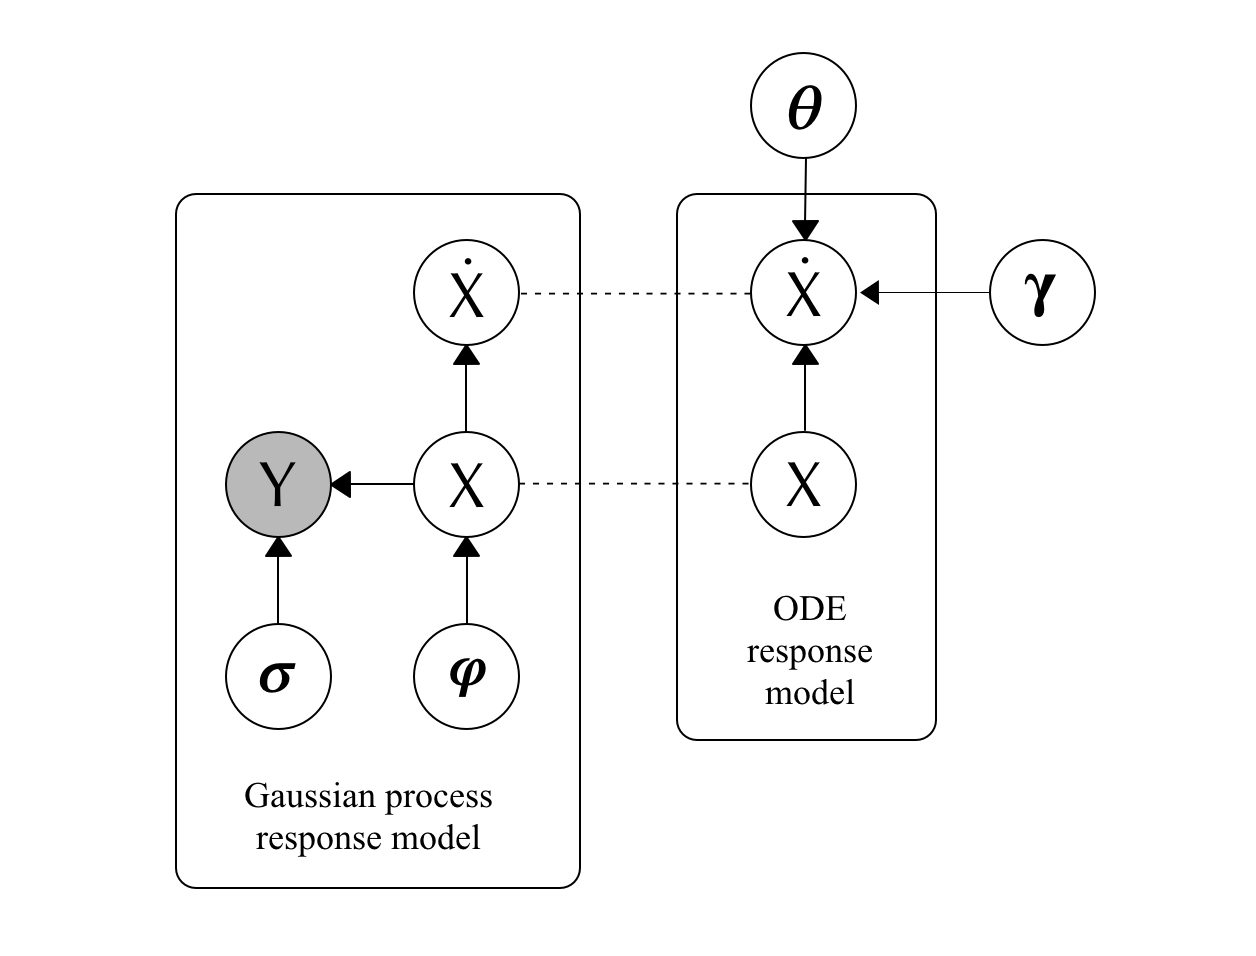
\includegraphics[width=0.8\textwidth]{graphics/gradient-matching-model}
    \caption{Graphical representation of the gradient matching with Gaussian processes model proposed by \cite{calderhead2009accelerating}. The dashed lines indicate information association from two response models using the product of experts \refequationp{\ref{eq-gmgp-poe}} . Details of the model are in \refsection{\ref{sec-sampling-gradient-matching}}.}    
    \label{fig-gmgp-model}
\end{figure}

\subsubsection*{Original sampling scheme}

\cite{calderhead2009accelerating} propose to integrate over the latent state derivatives $\dymdX$ to obtain
\begin{align}
    p(\dymtheta,\dymgamma\vert\dymX,\dymphi) 
    & =
    p(\dymtheta) p(\dymgamma) \int{
        p(\dymdX\vert\dymX,\dymtheta,\dymphi,\dymgamma)d\dymdX}
    \nonumber
    \\
    & \propto
    \frac{p(\dymtheta) p(\dymgamma)}{\mathcal{Z}(\dymgamma)} 
    \exp{[
        -\frac{1}{2}\sum_k{
            (\dymfkXshort{k} - \dymmk{k})^T\dymLambdak{k}(\dymfkXshort{k} - \dymmk{k})}]}
\end{align}
where $\dyminvLambdak{k} = \dymAk{k} + \dymgammak{k}\mI$, $\mathcal{Z}(\dymgamma) = \prod_k \lvert 2\pi(\dymAk{k} + \dymgammak{k}\mI) \rvert^{\frac{1}{2}}$ and $\dymfkXshort{k} = \dymfkX{k}$.

Then the sampling procedure follows the scheme below
\begin{align}
    \dymphi,\dymsigma 
    & \sim p(\dymphi,\dymsigma\vert\dymY)
    \label{eq-gmgp-sample-1}
    \\
    \dymX 
    & \sim p(\dymX\vert\dymY,\dymphi,\dymsigma)
    \label{eq-gmgp-sample-2}
    \\
    \dymtheta,\dymgamma 
    & \sim p(\dymtheta,\dymgamma\vert\dymX,\dymphi)
    \label{eq-gmgp-sample-3}    
\end{align}
where 
\begin{align}
    p(\dymphi, \dymsigma\vert\dymY) 
    & \propto p(\dymphi)p(\dymsigma)p(\dymY\vert\dymphi,\dymsigma) 
    \nonumber
    \\
    & \propto p(\dymphi)p(\dymsigma)\int{p(\dymX\vert\dymphi)p(\dymY\vert\dymX,\dymsigma)d\dymX}
    \nonumber
    \\
    & = p(\dymphi)p(\dymsigma)\prod_k{\mathcal{N}(\dymyk{k}\vert\mvector{0}, \dymCphik{k} + \dymsigmak{k}^2\mI)}    
    \nonumber
\end{align}

The sampling procedure requires two MCMC samplings for \refequationp{\ref{eq-gmgp-sample-1}} and \refequationp{\ref{eq-gmgp-sample-3}} respectively, and a direct sampling from the multivariate Gaussian distribution in \refequationp{\ref{eq-gmgp-sample-2}}.
The sampling steps are repeated until convergence is reached.

\subsubsection*{Adaptive sampling scheme}
One fundamental weakness of the previous sampling strategy is that the results on $\dymtheta$ and $\dymgamma$ from \refequationp{\ref{eq-gmgp-sample-3}} are never propagated back to \refequationp{\ref{eq-gmgp-sample-1}} and \refequationp{\ref{eq-gmgp-sample-2}}, and hence have no influence on the inference of states $\dymX$.
To close the feedback loop, \cite{dondelinger2013ode} proposed an improved sampling scheme called \emph{adaptive gradient matching}.

\cite{dondelinger2013ode} consider the joint distribution $p(\dymdX,\dymX,\dymphi,\dymtheta,\dymgamma)$, and show that its marginalization over the state derivatives $\dymdX$ is tractable:
\begin{align}
    p(\dymX,\dymphi,\dymtheta,\dymgamma)
    & = \int{
        p(\dymdX,\dymX,\dymphi,\dymtheta,\dymgamma) d\dymdX
        }
    \nonumber
    \\
    & = p(\dymX\vert\dymphi) p(\dymphi) p(\dymtheta) p(\dymgamma) \int{
        p(\dymdX\vert\dymX,\dymphi,\dymtheta,\dymgamma) d\dymdX}
    \nonumber
    \\
    & \propto \exp{[
        -\frac{1}{2}\sum_k{
            (\dymxk{k}^T\dyminvCphik{k}\dymxk{k} + (\dymfkXshort{k} - \dymmk{k})^T\dymLambdak{k}(\dymfkXshort{k} - \dymmk{k}))}]}
\end{align}

The full joint distribution, after integrating over the latent state derivatives $\dymdX$, is then given by
\begin{align}
    p(\dymY, \dymX, \dymphi, \dymtheta, \dymsigma, \dymgamma)
    & = p(\dymY\vert\dymX,\dymsigma) p(\dymX|\dymphi, \dymtheta, \dymgamma) p(\dymphi) p(\dymtheta) p(\dymsigma) p(\dymgamma)
    \nonumber
    \\
    & = p(\dymY\vert\dymX,\dymsigma) p(\dymX,\dymphi,\dymtheta,\dymgamma) p(\dymsigma)    
\end{align}

Based on the above joint distribution, \cite{dondelinger2013ode} devised an improved Metropolis-Hastings sampling scheme, which allows $\dymtheta$ to exert an influence on $\dymX$.

\subsubsection*{Summary}

To conclude this section, given the implicit solutions from the Gaussian processes, the states and parameters of the ODEs are inferred simultaneously without explicitly solving the ODEs anymore, which has led to significant speed-up.
Lastly, \cite{calderhead2009accelerating} also discuss the handling of partial observations, i.e.\ when some states are not observed, by utilizing to the prior we have imposed on the states \refequationp{\ref{eq-gmgp-x-prior}}.

\section{Variational gradient matching with Gaussian processes}
\label{sec-variational-gradient-matching}

Instead of using sampling methods, \cite{gorbach2016mean, gorbach2017scalable} proposed a solution to the previous problem based on variational inference, which has been shown, for specific types of ODEs \refequationp{\ref{eq-vgmgp-odes}} as discussed below, to be much more efficient than the sampling-based solutions, and scales well to large dynamical systems such the deterministic Lorenz 96 model with $1000$ states in their experiments.
This section gives an outline of the method by following the description from \cite{gorbach2017scalable} and the method is abbreviated as \algovgmgp\ in the rest of this work.

\subsubsection*{Maximum a posteriori estimation}

By combining the prior $p(\dymtheta)$, the state posterior  \refequationp{\ref{eq-gmgp-x-posterior}}, the product of experts result \refequationp{\ref{eq-gmgp-poe}}, and then integrating out the latent state derivatives $\dymdX$ as in \cite{calderhead2009accelerating}, the joint posterior $p(\dymX,\dymtheta\vert\dymY,\dymphi,\dymsigma,\dymgamma)$ is given as follows:
\begin{align}
    p(\dymX,\dymtheta\vert\dymY,\dymphi,\dymsigma,\dymgamma) 
    & = 
    p(\dymtheta)\int{
        p(\dymX\vert\dymY,\dymphi,\dymsigma) p(\dymdX\vert\dymX,\dymtheta,\dymphi,\dymgamma) d\dymdX
    }
    \nonumber
    \\
    & \propto
    p(\dymtheta) \prod_k{[
        \mathcal{N}(\dymxk{k}\vert\dymmuk{k}, \dymSigmak{k}) 
        \mathcal{N}(\dymfkX{k}\vert\dymmk{k},\dyminvLambdak{k})]}    
    \label{eq-vgmgp-posterior-joint}
\end{align}

Using the inference of the parameters $\dymtheta$ as an example, the ``best'' parameters $\dymtheta^*$ could ideally be estimated based on the \emph{maximum a posteriori (MAP)} of the posterior $p(\dymtheta\vert\dymY,\dymphi,\dymsigma,\dymgamma)$, which is equivalent to
\begin{align}
    \dymtheta^* = \argmax_{\dymtheta}\ln{p(\dymtheta\vert\dymY,\dymphi,\dymsigma,\dymgamma)}
    \label{eq-vgmgp-theta-posterior}
\end{align}
where the posterior on $\dymtheta$ is obtained by marginalizing \refequationp{\ref{eq-vgmgp-posterior-joint}} over the states $\dymX$, namely
\begin{align}
    p(\dymtheta\vert\dymY,\dymphi,\dymsigma,\dymgamma) = \int{p(\dymX,\dymtheta\vert\dymY,\dymphi,\dymsigma,\dymgamma)d\dymX}
    \nonumber
\end{align} 

However, the above equation is intractable due to strong non-linear couplings of the states induced by the ODEs \refequationp{\ref{eq-gmgp-odes}}.
As a workaround, \cite{gorbach2017scalable} designed a proxy distribution on the states and parameters denoted as $Q(\dymX, \dymtheta)$, and derived analytically tractable variational lower bounds based on mean-field variational inference.

\subsubsection*{Structural assumption}

First of all, the ODEs primarily considered by \cite{gorbach2017scalable} are state-wise of the following structure:
\begin{align}
    \dymfk{k} = \sum_m{\dymthetam{m}\prod_{i\in\mathcal{M}_{km}}{\dymxktn{i}{}}} + C
    \label{eq-vgmgp-odes}\
\end{align}
for $k = \mrange{1}{K}$, where $\mathcal{M}_{km}$ contains the states in the $k$-th equation of the ODEs that are controlled by the $m$-th parameter $\dymthetam{m}$, and $C$ denotes other terms that are independent of the parameters.
The first term of \refequationp{\ref{eq-vgmgp-odes}} can be viewed as a linear combination of the parameters and the product of the monomials of the states.
For the second term, the only requirement on terms in $C$ is that each state can only appear as monomial inside a term, but a term in $C$ can contain the product of the monomials of the states.

The structural assumption imposed on the ODEs leads to an important conclusion that the  following conditional distributions $p(\dymtheta\vert\dymY,\dymX,\dymphi,\dymgamma)$ and $p(\dymxk{u}\vert\dymY,\dymXwithoutk{u},\dymphi,\dymtheta,\dymsigma,\dymgamma)$ for $u = \mrange{1}{K}$ are Gaussian distributed, where $\dymXwithoutk{u} = \{\dymxk{o}\vert o = \mrange{1}{K}\ \text{and}\ o \neq u \}$, i.e.\ $\dymXwithoutk{u}$ is the set of all states except $\dymxk{u}$. 
But before writing out the distributions, we first need to introduce several more notations. 

One implication of the above assumption is that each ODE can be expressed as a linear combination of the parameters plus a term that is independent of them.
We therefore use $\dymBthetakX{k}$ and $\dymbthetakX{k}$ to denote the corresponding coefficients such that $\dymBthetakX{k}\dymtheta + \dymbthetakX{k} = \dymfkX{k}$ for $k = \mrange{1}{K}$.
Similarly, due to the monomial assumption about the states, each ODE can also be transformed into a linear combination of the $u$-th state for $u = \mrange{1}{K}$ plus an independent term.
Here we adopt the terms $\dymBukX{k}$ and $\dymbukX{k}$ to denote the respective coefficients such that $\dymBukX{k}\dymxk{u} + \dymbukX{k} = \dymfkX{k}$ for $k,u = \mrange{1}{k}$.

With these notations, we now state the conditional distributions $p(\dymtheta\vert\dymY,\dymX,\dymphi,\dymgamma)$ and $p(\dymxk{u}\vert\dymY,\dymXwithoutk{u},\dymphi,\dymtheta,\dymsigma,\dymgamma)$ as follows:
\begin{align}
    p(\dymtheta\vert\dymY,\dymX,\dymphi,\dymgamma)
    & = \mathcal{N}(\dymtheta\vert\dymrtheta, \dymOmegatheta)    
    \label{eq-vgmgp-theta-conditional}
    \\
    p(\dymxk{u}\vert\dymY,\dymXwithoutk{u},\dymphi,\dymtheta,\dymsigma,\dymgamma)
    & = \mathcal{N}(\dymxk{u}\vert\dymru, \dymOmegau)
    \label{eq-vgmgp-xu-conditional}
\end{align}
where 
\begin{align}
    \dymrtheta 
    & = \dymOmegatheta \sum_k{\dymBthetakX{k}^T\dymLambdak{k}(\dymmk{k} - \dymbthetakX{k})}    
    \label{eq-vgmgp-theta-conditional-mean}
    \\
    \dyminvOmegatheta
    & = \sum_k{\dymBthetakX{k}^T\dymLambdak{k}\dymBthetakX{k}}
    \label{eq-vgmgp-theta-conditional-covariance}
    \\
    \dymru
    & = \dymOmegau[
        \dyminvSigmak{u}\dymmuk{u}
        + \sum_k{
            \dymBukX{k}^T\dymLambdak{k}(\dymmk{k} - \dymbukX{k})}        
    ]
    \label{eq-vgmgp-xu-conditional-mean}
    \\
    \dyminvOmegau
    & = \dyminvSigmak{u} + \sum_k{
        \dymBukX{k}^T\dymLambdak{k}\dymBukX{k} 
    } 
    \label{eq-vgmgp-xu-conditional-covariance}
\end{align}
The proofs are omitted here and can be found in the supporting materials of \cite{gorbach2017scalable}.
They basically utilizes the formula to calculate the product of Gaussians \citep[\refsection{8.1}]{petersen2012matrix}, and the well-known closure property of Gaussian distribution under linear transformations, to obtain a closed-form solution.
As a side note, this conclusion will also be used later in \refchapter{\ref{ch-laplace-approximation}} to derive another approximate inference solution based on the Laplace approximation technique.

To simplify the notations, in the following, we will switch to the canonical form of \emph{exponential family} \citep[\refsection{9.2}]{murphy2012machine} to describe the distributions \refequationp{\ref{eq-vgmgp-theta-conditional}} and \refequationp{\ref{eq-vgmgp-xu-conditional}} as:
\begin{align}
    p(\dymtheta\vert\dymY,\dymX,\dymphi,\dymgamma)
    & = \dymhthetacanonical \exp{(\dymetathetacanonical^T\dymTthetacanonical - \dymAthetacanonical)}
    \label{eq-vgmgp-theta-conditional-canonical}
    \\
    p(\dymxk{u}\vert\dymY,\dymXwithoutk{u},\dymphi,\dymtheta,\dymsigma,\dymgamma)
    & = \dymhucanonical \exp{(\dymetaucanonical^T\dymTucanonical - \dymAucanonical)}
    \label{eq-vgmgp-xu-conditional-canonical}
\end{align}
where $\dymetacanonical, \dymTcanonical, \dymhcanonical, \dymAcanonical$ are the \emph{natural parameters}, \emph{sufficient statistics},  \emph{base measure} and \emph{log partition function} respectively .

\subsubsection*{Variational lower bound}

Introducing $\dymlambdavi$ and $\dympsiuvi$ for $u = \mrange{1}{K}$ as the variational parameters, the proxy distribution $Q(\dymX,\dymtheta)$ is constrained to the family $\mathcal{Q}$ that factorizes over the parameters and the states, and each factor is in the same exponential family as its corresponding counterparts defined in  \refequationp{\ref{eq-vgmgp-theta-conditional-canonical}} and \refequationp{\ref{eq-vgmgp-xu-conditional-canonical}} such that
\begin{align}
    \mathcal{Q} 
    & = \{
        Q(\dymX,\dymtheta)\vert Q(\dymX,\dymtheta) = q(\dymtheta\vert\dymlambdavi)\prod_u{q(\dymxk{u} \vert\dympsiuvi)}\}
    \label{eq-vgmgp-proxy-family}
    \intertext{where}
    q(\dymtheta\vert\dymlambdavi)
    & = \dymhthetacanonicalQ \exp{(
        \dymlambdavi^T\dymTthetacanonicalQ - \dymAthetacanonicalQ)}
    \nonumber
    \\
    q(\dymxk{u}\vert\dympsiuvi)
    & = \dymhucanonicalQ \exp{(
        \dympsiuvi^T\dymTucanonicalQ - \dymAucanonicalQ)}
    \nonumber
\end{align}

Using standard mean-field variation technique, the optimal $Q^*$ is given by
\begin{align}
    Q^* 
    & = \argmin_{Q(\dymX,\dymtheta)\in\mathcal{Q}}KL(Q(\dymX,\dymtheta)\|p(\dymX,\dymtheta\vert\dymY,\dymphi,\dymsigma,\dymgamma)) 
    \nonumber
    \\
    & = \argmax_{Q(\dymX,\dymtheta)\in\mathcal{Q}}\mathcal{L}_Q(\dymlambdavi,\dympsivi)
\end{align}
where $\mathcal{L}_Q(\dymlambdavi,\dympsivi)$ denotes the evidence lower bound.

\cite{gorbach2017scalable} showed that maximizing $\mathcal{L}_Q(\dymlambdavi,\dympsivi)$ with respect to $\dymtheta$ is equivalent to maximizing
\begin{align}
    \mathcal{L}_{\dymtheta}(\dymlambdavi) 
    & = \mathbb{E}_Q[
            \ln{p(\dymtheta\vert\dymY,\dymX,\dymphi,\dymgamma)}]
        - \mathbb{E}_Q[
            \ln{q(\dymtheta\vert\dymlambdavi)}]
    \nonumber             
    \\
    & = \mathbb{E}_Q[
        \dymetathetacanonical^T\nabla_{\dymlambdavi}\dymAthetacanonical] - \dymlambdavi^T\nabla_{\dymlambdavi}\dymAthetacanonicalQ
    \label{eq-vgmgp-elbo-theta}
\end{align}
and maximizing $\mathcal{L}_Q(\dymlambdavi,\dympsivi)$ with respect to $\dymxk{u}$ is equivalent to maximizing
\begin{align}
    \mathcal{L}_{\dympsiuvi} 
    & = \mathbb{E}_Q[
            \ln{p(\dymxk{u}\vert\dymY,\dymXwithoutk{u},\dymphi,\dymtheta,\dymsigma,\dymgamma)}]
        - \mathbb{E}_Q[
            \ln{q(\dymxk{u}\vert\dympsiuvi)}
        ]
    \nonumber
    \\
    & = \mathbb{E}_Q[
        \dymetaucanonical^T\nabla_{u}\dymAucanonical] -\dympsiuvi^T\nabla_{u}\dymAucanonicalQ
    \label{eq-vgmgp-elbo-xu}
\end{align}
where $\nabla_{(\cdot)}$ is the gradient operator.

Given the assumption about the conditional distributions \refequationp{\ref{eq-vgmgp-theta-conditional-canonical}} and \refequationp{\ref{eq-vgmgp-xu-conditional-canonical}}, plus the design of the proxy distribution family \refequationp{\ref{eq-vgmgp-proxy-family}}, they further showed that the lower bounds \refequationp{\ref{eq-vgmgp-elbo-theta}} and \refequationp{\ref{eq-vgmgp-elbo-xu}} can be optimized analytically by setting their gradients  with respect to their variational parameters to zero. 
The optimal variational parameters are thus given by
\begin{align}
    \dymlambdavi^*
    & = \mathbb{E}_Q[\dymetathetacanonical] 
    \label{eq-vgmgp-lambda-vi-optimal}
    \\
    \dympsiuvi^* 
    & = \mathbb{E}_Q[\dymetaucanonical]
    \label{eq-vgmgp-psiu-vi-optimal}
\end{align}
where the natural parameters are defined as $\dymetathetacanonical = [\dyminvOmegatheta\dymrtheta, -\frac{1}{2}\dyminvOmegatheta]^T$ and $\dymetaucanonical = [\dyminvOmegau \dymru, -\frac{1}{2}\dyminvOmegau]^T$.

\subsection*{\algovgmgp\ algorithm}

\begin{algorithm}
    \centering
    \caption{Pseudocode for the \algovgmgp\ algorithm.}
    \label{algo-vgmgp}
    \begin{algorithmic}[1]
        \For{$u = \mrange{1}{K}$}
            \State 
            \text{Initialize $\dymmuk{u}$, $\dymSigmak{u}$, $\dymmk{u}$ and $\dymLambdak{u}$ using Gaussian process regression}
        \EndFor
        \State
        \While{\text{not converged or maximum iteration not reached}}            
            \For{$u = \mrange{1}{K}$}
                \State 
                \text{Update the mean and variance of $\hat{q}_{\dympsiuvi}$ using $\mvector{\hat{\theta}}^{(i)}$}
            \EndFor                
            
            \State 
            \text{$\mvector{\hat{\theta}}^{(i+1)} = \argmax_{\dymtheta}{\mathbb{E}_Q[\sum_k{\ln{\mathcal{N}(\dymfkX{k}\vert\dymmk{k},\dyminvLambdak{k})}}]}$}
        \EndWhile
    \end{algorithmic}
\end{algorithm}

To close this section, the pseudocode of their algorithm is summarized in \refalgorithm{\ref{algo-vgmgp}}.
The algorithm first uses Gaussian process regression to obtain a smoothed estimate for the states and the distribution on the state derivatives.
As noted by \cite{gorbach2017scalable}, the Gaussian process priors come in naturally in cases where there exist unobserved states.

In the second step, the algorithm uses the variational gradient matching framework described before to maximize the lower bounds iteratively.
In every iteration, the states and parameters are optimized in an \emph{expectation-maximization (EM)} \cite[\refsection{9.4}]{bishop2006pattern} fashion until convergence is reached or the maximum allowed number of iterations is reached.



